\documentclass{beamer}

\usetheme{shadow} %Copenhagen %Luebeck % shadow 100% confirmed

\title{Gettysburg Cemetery Dedication}
\author{Abraham Lincoln}
\institute{United States of America}
\date{19 Nov 1863}

\begin{document}

\begin{frame}
  \titlepage
\end{frame}

\begin{frame}{Outline}
  
\end{frame}

\begin{frame}{Agenda}
\begin{itemize}
    \item Met on battlefield (great)
    \item Dedicate portion of field --- fitting!
    \item Unfinished work (great tasks)
\end{itemize}
\end{frame}

\begin{frame}{Not on Agenda!}
\begin{itemize}
    \item Dedicate
    \pause \item Consecrate
    \pause \item Hallow (in narrow sense)
    \pause \item Add or detract
    \pause \item Note or remember what we say
\end{itemize}
\end{frame}

\begin{frame}{Key Objectives \& Success Factors}
\begin{itemize}
    \item What makes nation unique:
    \begin{itemize}
    \item Conceived in Liberty
    \item Men are equal
    \end{itemize}
\end{itemize}

\begin{block}{Shared vision:}
\begin{itemize}
  \item New birth of freedom.
  \item Gov't of/for/by the people.
\end{itemize}
\end{block}
\end{frame}

\begin{frame}{Organizational Overview}
\begin{align*}
    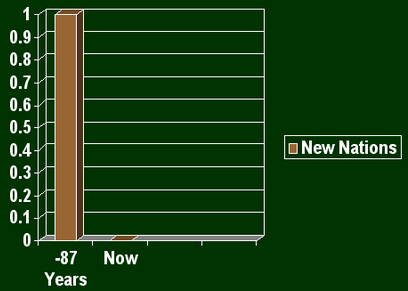
\includegraphics[width=0.5\textwidth]{Resources/gettysburg_graph.png}
\end{align*}

\begin{block}{Four Score and Seven}
\begin{equation}
-(4 * 20 + 7) = -87
\end{equation}
\end{block}
\end{frame}

\begin{frame}{Summary}
\begin{columns}
\begin{column}{0.5\textwidth}
\begin{itemize}
  \item New nation
  \item Civil war
  \item Dedicate field
\end{itemize}
\end{column}
\begin{column}{0.5\textwidth}
\begin{itemize}
  \item Dedicated to unfinished work
  \item New birth of freedom
  \item Government not perish
\end{itemize}
\end{column}
\end{columns}
\end{frame}

\end{document}